\section{Use Cases Model}
\label{sec:lu.uni.lassy.excalibur.group01.excalibur-gendescr-usecasemodel}

This section contains the use cases elicited during the requirements elicitation phase.
The use cases are textually described as suggested by the \msrmessir method and inspired by the standard Cokburn template~\cite{armour01usecase}.


%% ***************************************************************
%% Use Cases
\subsection{Use Cases}



%% ***************************************************************
%% Summary Use Cases



%% ***************************************************************
%% User-Goal Use Cases
\subsubsection{usergoal-ugAddRoom}

\label{RE-use-case-ugAddRoom}


The goal is to add a new Room to the room database.		  


\begin{usecase}
  \addheading{Use-Case Description}
  \addsingletwocolumnrow{Name}{ugAddRoom}
  \addsingletwocolumnrow{Scope}{system}
  \addsingletwocolumnrow{Level}{usergoal}
  

\addrowheading{Primary actor(s)}
\addnumberedsinglerow{}{\msrcode{actManager[active]}}



\addrowheading{Goal(s) description}
\addsinglerow{The goal is to add a new Room to the room database.}

\addrowheading{Reuse}
\addnumberedsinglerow{}{\msrucname{sfEnterFields [0..*]}}
\addnumberedsinglerow{}{\msrucname{sfAddRoom [0..*]}}

\addrowheading{Protocol condition(s)}
\addnumberedsinglerow{}{
}

\addrowheading{Pre-condition(s)}
\addnumberedsinglerow{}{
The user needs to be a manager to be able to add a new room.
}

\addrowheading{Main post-condition(s)}
\addnumberedsinglerow{}{
The new room is added to the database.
}

\addrowheading{Main Steps}
\addalphanumberedsinglerow{}{the actor \msrcode{actManager} executes the \msrucname{sfEnterFields} use case}
\addalphanumberedsinglerow{}{the actor \msrcode{actManager} executes the \msrucname{sfAddRoom} use case}

\addrowheading{Additional Information}
\addsinglerow{
none
}

\end{usecase} 


Figure \ref{fig:lu.uni.lassy.excalibur.group01.excalibur-RE-UCD-ugAddRoom}
The manager has the ability to add a room.

\begin{figure}[htbp]
\begin{center}

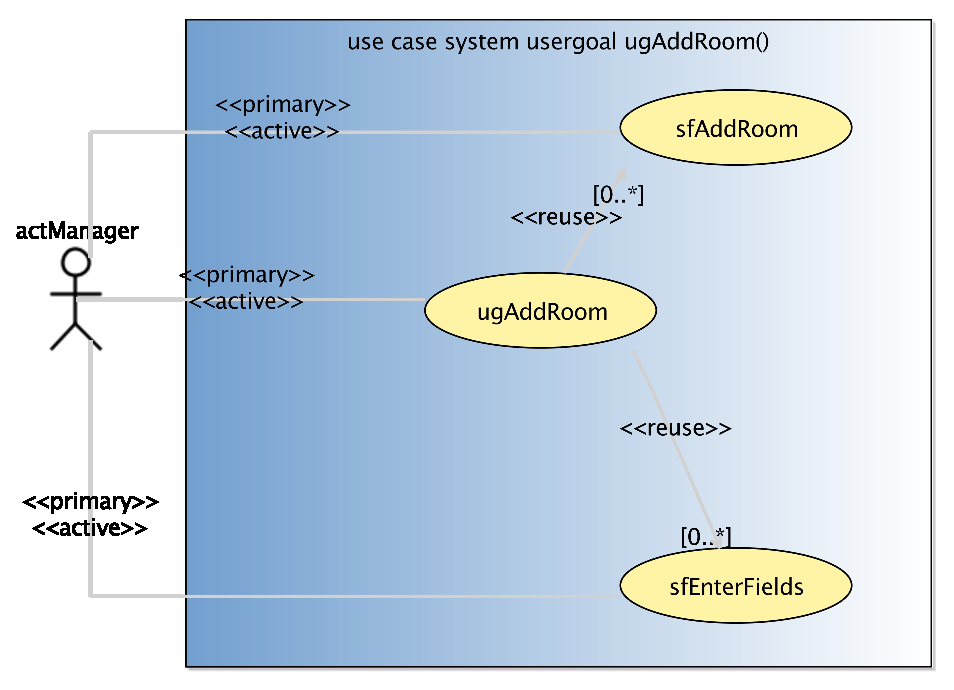
\includegraphics[
angle=0
]{./images-report-gen/usecase-model/usergoal/ugAddRoom.eps}
\end{center}
\caption[lu.uni.lassy.excalibur.group01.excalibur Use Case Diagram: ugAddRoom]{Add Room Function for the Manager Actor}
\label{fig:lu.uni.lassy.excalibur.group01.excalibur-RE-UCD-ugAddRoom}
\end{figure}
\vspace{0.5cm}

\subsubsection{usergoal-ugAskForFruitOrVegtable}

\label{RE-use-case-ugAskForFruitOrVegtable}


The gardener has the ability to ask for a new fruit or vegetable		  


\begin{usecase}
  \addheading{Use-Case Description}
  \addsingletwocolumnrow{Name}{ugAskForFruitOrVegtable}
  \addsingletwocolumnrow{Scope}{system}
  \addsingletwocolumnrow{Level}{usergoal}
  

\addrowheading{Primary actor(s)}
\addnumberedsinglerow{}{\msrcode{actGardener[active]}}



\addrowheading{Goal(s) description}
\addsinglerow{The gardener has the ability to ask for a new fruit or vegetable}


\addrowheading{Protocol condition(s)}
\addnumberedsinglerow{}{
}

\addrowheading{Pre-condition(s)}
\addnumberedsinglerow{}{
The gardener has to be logged in and has to be on his home screen.
}

\addrowheading{Main post-condition(s)}
\addnumberedsinglerow{}{
The request has been send to the manger.
}


\addrowheading{Additional Information}
\addsinglerow{
There are no constraints on the demand but there is a pop up which appears which has to be accepted to successfully
send the request.
}

\end{usecase} 


\subsubsection{usergoal-ugAskForSensor}

\label{RE-use-case-ugAskForSensor}


The Technician goal is to request a sensor type to the manager.		  


\begin{usecase}
  \addheading{Use-Case Description}
  \addsingletwocolumnrow{Name}{ugAskForSensor}
  \addsingletwocolumnrow{Scope}{system}
  \addsingletwocolumnrow{Level}{usergoal}
  

\addrowheading{Primary actor(s)}
\addnumberedsinglerow{}{\msrcode{actTechnician[active]}}



\addrowheading{Goal(s) description}
\addsinglerow{The Technician goal is to request a sensor type to the manager.}

\addrowheading{Reuse}
\addnumberedsinglerow{}{\msrucname{oeEntersFields [1..1]}}
\addnumberedsinglerow{}{\msrucname{suRequestItem [1..1]}}

\addrowheading{Protocol condition(s)}
\addnumberedsinglerow{}{
}

\addrowheading{Pre-condition(s)}
\addnumberedsinglerow{}{
The gardener has to be logged in the system.
}

\addrowheading{Main post-condition(s)}
\addnumberedsinglerow{}{
The table request from manager is updated
}

\addrowheading{Main Steps}
\addalphanumberedsinglerow{}{the actor \msrcode{actTechnician} executes the \msrucname{oeEntersFields} use case}
\addalphanumberedsinglerow{}{the actor \msrcode{actTechnician} executes the \msrucname{suRequestItem} use case}

\addrowheading{Additional Information}
\addsinglerow{
none
}

\end{usecase} 


Figure \ref{fig:lu.uni.lassy.excalibur.group01.excalibur-RE-UCD-ugAskForSensor}
The technician has the ability to request a sensor

\begin{figure}[htbp]
\begin{center}

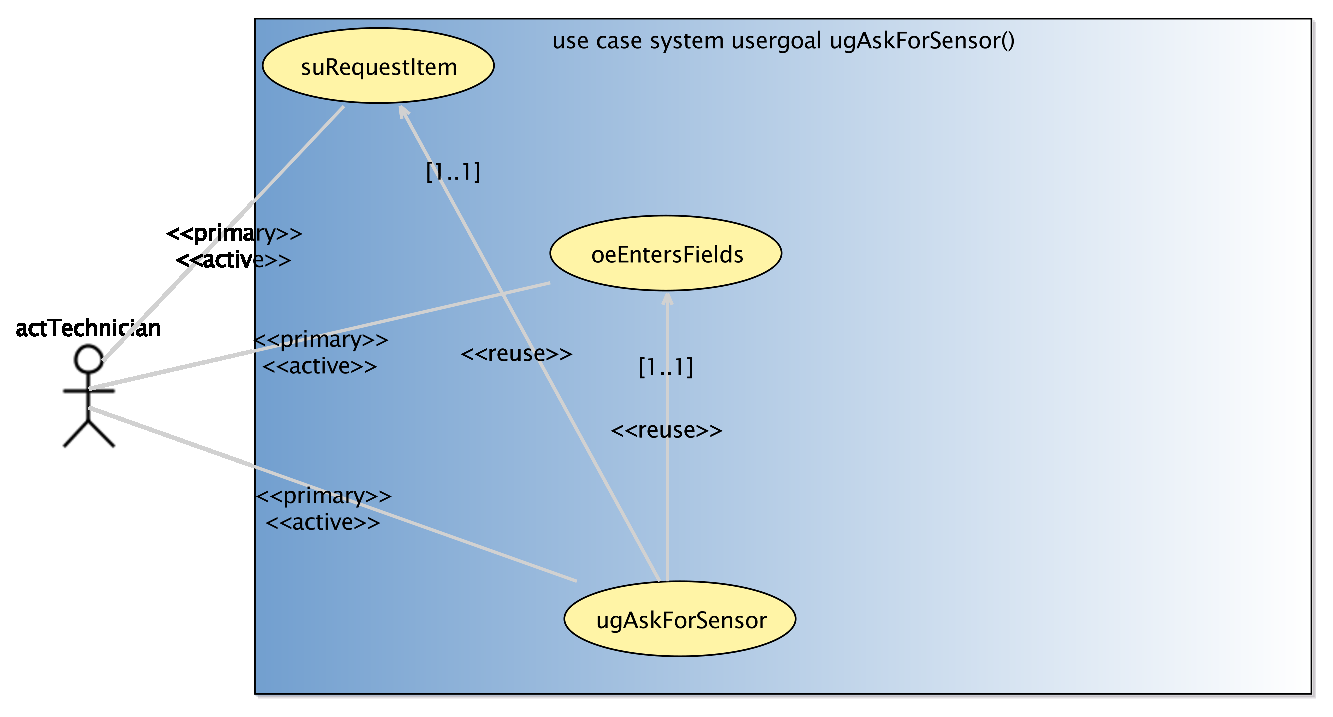
\includegraphics[
angle=0
]{./images-report-gen/usecase-model/usergoal/ugAskForSensor.eps}
\end{center}
\caption[lu.uni.lassy.excalibur.group01.excalibur Use Case Diagram: ugAskForSensor]{Technician requests sensor}
\label{fig:lu.uni.lassy.excalibur.group01.excalibur-RE-UCD-ugAskForSensor}
\end{figure}
\vspace{0.5cm}

\subsubsection{usergoal-ugFillingGardnerSchedule}

\label{RE-use-case-ugFillingGardnerSchedule}


The goal is it to qdd tasks to the schedule		  


\begin{usecase}
  \addheading{Use-Case Description}
  \addsingletwocolumnrow{Name}{ugFillingGardnerSchedule}
  \addsingletwocolumnrow{Scope}{system}
  \addsingletwocolumnrow{Level}{usergoal}
  

\addrowheading{Primary actor(s)}
\addnumberedsinglerow{}{\msrcode{actManager[active]}}



\addrowheading{Goal(s) description}
\addsinglerow{The goal is it to qdd tasks to the schedule}

\addrowheading{Reuse}
\addnumberedsinglerow{}{\msrucname{sfFillingTextFields [0..*]}}
\addnumberedsinglerow{}{\msrucname{sfChooseImportance [0..1]}}

\addrowheading{Protocol condition(s)}
\addnumberedsinglerow{}{
}

\addrowheading{Pre-condition(s)}
\addnumberedsinglerow{}{
Manager must be securly logined and be on the manager screen.
}

\addrowheading{Main post-condition(s)}
\addnumberedsinglerow{}{
Schedule has an additonal task more tasks
}

\addrowheading{Main Steps}
\addalphanumberedsinglerow{}{the actor \msrcode{actManager} executes the \msrucname{sfEnterFields} use case}
\addalphanumberedsinglerow{}{the actor \msrcode{actManager} executes the \msrucname{sfChooseImportance} use case}

\addrowheading{Additional Information}
\addsinglerow{
The input has to be write no sanity checks are done.
}

\end{usecase} 


Figure \ref{fig:lu.uni.lassy.excalibur.group01.excalibur-RE-UCD-ugFillingGardnerSchedule}
The goal is it to add a task to the schedule

\begin{figure}[htbp]
\begin{center}

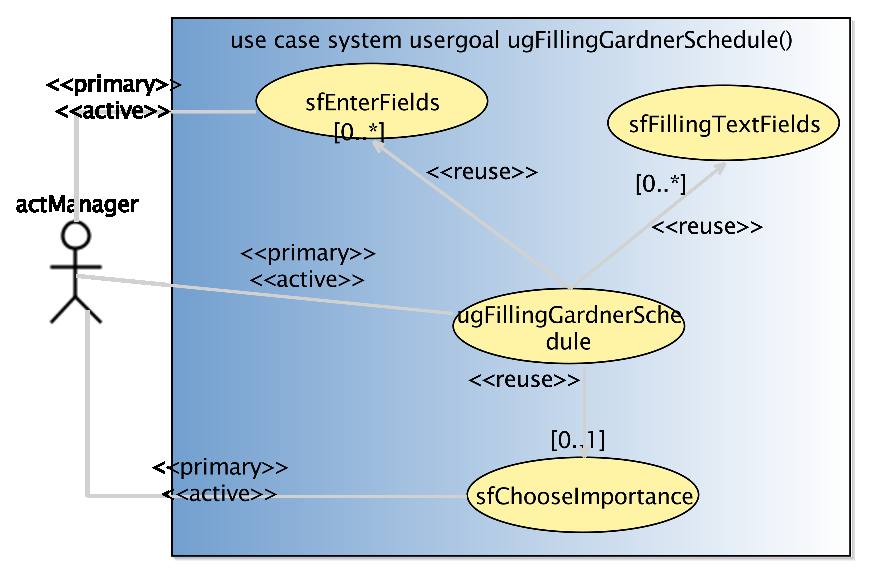
\includegraphics[
angle=0
]{./images-report-gen/usecase-model/usergoal/ugFillingGardnerSchedule.eps}
\end{center}
\caption[lu.uni.lassy.excalibur.group01.excalibur Use Case Diagram: ugFillingGardnerSchedule]{Adding task to schedule}
\label{fig:lu.uni.lassy.excalibur.group01.excalibur-RE-UCD-ugFillingGardnerSchedule}
\end{figure}
\vspace{0.5cm}

\subsubsection{usergoal-ugSecurelyUseSystem}

\label{RE-use-case-ugSecurelyUseSystem}


Every actor has the possibility to connect to the system but no other person from outside		  


\begin{usecase}
  \addheading{Use-Case Description}
  \addsingletwocolumnrow{Name}{ugSecurelyUseSystem}
  \addsingletwocolumnrow{Scope}{system}
  \addsingletwocolumnrow{Level}{usergoal}
  

\addrowheading{Primary actor(s)}
\addnumberedsinglerow{}{\msrcode{actUser[active]}}



\addrowheading{Goal(s) description}
\addsinglerow{Every actor has the possibility to connect to the system but no other person from outside}

\addrowheading{Reuse}
\addnumberedsinglerow{}{\msrucname{oeLogin [1..1]}}
\addnumberedsinglerow{}{\msrucname{oeLogout [1..1]}}

\addrowheading{Protocol condition(s)}
\addnumberedsinglerow{}{
}

\addrowheading{Pre-condition(s)}
\addnumberedsinglerow{}{
No actor has to be logged in.
}

\addrowheading{Main post-condition(s)}
\addnumberedsinglerow{}{
The given actor can execute he's tasks and can logout after.
}

\addrowheading{Main Steps}
\addalphanumberedsinglerow{}{the actor \msrcode{actUser} executes the \msrucname{oeLogin} use case}
\addalphanumberedsinglerow{}{the actor \msrcode{actUser} executes the \msrucname{oeLogout} use case}
\addrowheading{Steps Ordering Constraints}
\addnumberedsinglerow{}{step (a) must always precede step (b).}

\addrowheading{Additional Information}
\addsinglerow{
The given actor has to logout him self.
}

\end{usecase} 


Figure \ref{fig:lu.uni.lassy.excalibur.group01.excalibur-RE-UCD-ugSecurelyUseSystem}
A given actor can securely login in.

\begin{figure}[htbp]
\begin{center}

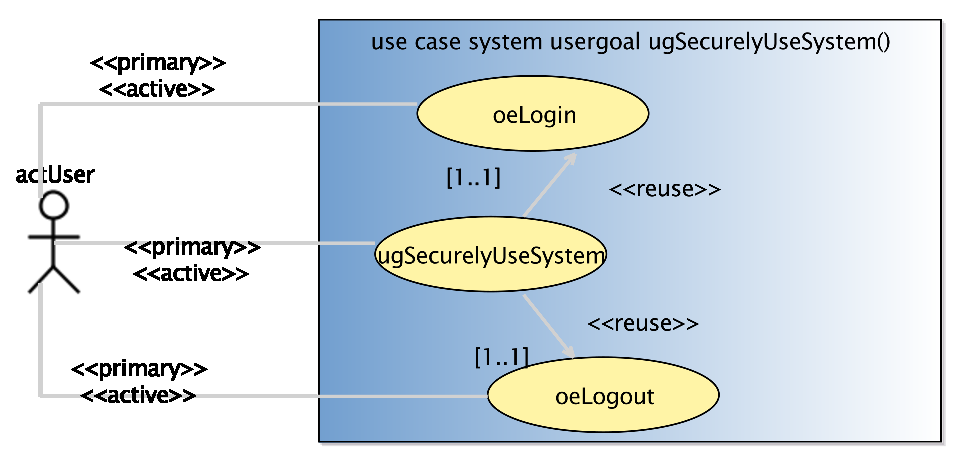
\includegraphics[
angle=0
]{./images-report-gen/usecase-model/usergoal/ugSecurelyUseSystem.eps}
\end{center}
\caption[lu.uni.lassy.excalibur.group01.excalibur Use Case Diagram: ugSecurelyUseSystem]{}
\label{fig:lu.uni.lassy.excalibur.group01.excalibur-RE-UCD-ugSecurelyUseSystem}
\end{figure}
\vspace{0.5cm}



%% ***************************************************************
%% Subfunction Use Cases
\subsubsection{subfunction-oeLogout}

\label{RE-use-case-oeLogout}


The currently signed in user is signed out by calling this function.		  


\begin{usecase}
  \addheading{Use-Case Description}
  \addsingletwocolumnrow{Name}{oeLogout}
  \addsingletwocolumnrow{Scope}{system}
  \addsingletwocolumnrow{Level}{subfunction}
  

\addrowheading{Primary actor(s)}
\addnumberedsinglerow{}{\msrcode{actUser[active]}}



\addrowheading{Goal(s) description}
\addsinglerow{The currently signed in user is signed out by calling this function.}

\addrowheading{Protocol condition(s)}
\addnumberedsinglerow{}{
}

\addrowheading{Pre-condition(s)}
\addnumberedsinglerow{}{
Actor is logged in.
}

\addrowheading{Main post-condition(s)}
\addnumberedsinglerow{}{
Actor is logged out.
}

\addrowheading{Additional Information}
\addsinglerow{
The actor has to be logged in. 
}

\end{usecase} 


\subsubsection{subfunction-sfAddRoom}

\label{RE-use-case-sfAddRoom}


This function add the entry into the room database.		  


\begin{usecase}
  \addheading{Use-Case Description}
  \addsingletwocolumnrow{Name}{sfAddRoom}
  \addsingletwocolumnrow{Scope}{system}
  \addsingletwocolumnrow{Level}{subfunction}
  

\addrowheading{Primary actor(s)}
\addnumberedsinglerow{}{\msrcode{actManager[active]}}



\addrowheading{Goal(s) description}
\addsinglerow{This function add the entry into the room database.}

\addrowheading{Protocol condition(s)}
\addnumberedsinglerow{}{
}

\addrowheading{Pre-condition(s)}
\addnumberedsinglerow{}{
The input formular needs to be correctly filled.
}

\addrowheading{Main post-condition(s)}
\addnumberedsinglerow{}{
The new room is now inside the room database.
}

\addrowheading{Additional Information}
\addsinglerow{
none
}

\end{usecase} 


\subsubsection{subfunction-sfEnterFields}

\label{RE-use-case-sfEnterFields}


The Manager needs to enter the different information for the new room to be added.		  


\begin{usecase}
  \addheading{Use-Case Description}
  \addsingletwocolumnrow{Name}{sfEnterFields}
  \addsingletwocolumnrow{Scope}{system}
  \addsingletwocolumnrow{Level}{subfunction}
  

\addrowheading{Primary actor(s)}
\addnumberedsinglerow{}{\msrcode{actManager[active]}}



\addrowheading{Goal(s) description}
\addsinglerow{The Manager needs to enter the different information for the new room to be added.}

\addrowheading{Protocol condition(s)}
\addnumberedsinglerow{}{
}

\addrowheading{Pre-condition(s)}
\addnumberedsinglerow{}{
All fields must be filled out correctly.
}

\addrowheading{Main post-condition(s)}
\addnumberedsinglerow{}{ 
The input fields get cleared and the new room is now added to the database
}

\addrowheading{Additional Information}
\addsinglerow{
Room name must be unique.
All other data must be numeric (Length, width, soil height)
}

\end{usecase} 


\subsubsection{subfunction-sfcheckSensor}

\label{RE-use-case-sfcheckSensor}


checksIfTheSensors are properly installed CHECK IF IT WORKS		  


\begin{usecase}
  \addheading{Use-Case Description}
  \addsingletwocolumnrow{Name}{sfcheckSensor}
  \addsingletwocolumnrow{Scope}{system}
  \addsingletwocolumnrow{Level}{subfunction}
  

\addrowheading{Primary actor(s)}
\addnumberedsinglerow{}{\msrcode{actTechnician[active]}}



\addrowheading{Goal(s) description}
\addsinglerow{checksIfTheSensors are properly installed CHECK IF IT WORKS}

\addrowheading{Protocol condition(s)}
\addnumberedsinglerow{}{
}

\addrowheading{Pre-condition(s)}
\addnumberedsinglerow{}{
}

\addrowheading{Main post-condition(s)}
\addnumberedsinglerow{}{
here is a post condition
}

\addrowheading{Additional Information}
\addsinglerow{
none
}

\end{usecase} 


\subsubsection{subfunction-sfplating}

\label{RE-use-case-sfplating}


plating the plants		  


\begin{usecase}
  \addheading{Use-Case Description}
  \addsingletwocolumnrow{Name}{sfplating}
  \addsingletwocolumnrow{Scope}{system}
  \addsingletwocolumnrow{Level}{subfunction}
  

\addrowheading{Primary actor(s)}
\addnumberedsinglerow{}{\msrcode{actGardener[active]}}



\addrowheading{Goal(s) description}
\addsinglerow{plating the plants}

\addrowheading{Protocol condition(s)}
\addnumberedsinglerow{}{
}

\addrowheading{Pre-condition(s)}
\addnumberedsinglerow{}{
Here is a preCondition
}

\addrowheading{Main post-condition(s)}
\addnumberedsinglerow{}{
}

\addrowheading{Additional Information}
\addsinglerow{
none
}

\end{usecase} 





%% ***************************************************************
%% Use Case Instances
\pagebreak
\subsection{Use Case Instance(s)}


%% ***************************************************************
%% Summary Use Case Instances



%% ***************************************************************
%% User-Goal Use Case Instances

	\subsubsection{Use-Case Instance - uciSecurelyUseSystem:ugSecurelyUseSystem}
	
	The view of the user		  
	\begin{operationmodel}
	\addheading{usergoal Use-Case Instance}
	\adddoublerow{Instantiated Use Case}{ugSecurelyUseSystem}
	\adddoublerow{Instance ID}{uciSecurelyUseSystem}
	
	\end{operationmodel} 

	




%% ***************************************************************
%% Subfunction Use Case Instances
